\chapter{Triển khai mô phỏng}

Linh kiện chưa về đủ thì thiết kế vẫn có thể chạy thử. Chương này dựng lại toàn bộ luồng dữ liệu của Haitay bằng phần mềm, từ cú chạm tay tới bảng trong SQLite, rồi đem nó qua các tình huống xấu mà chương trước đã đề phòng. Kết quả là bằng chứng đầu tiên cho thấy ba bất biến của luồng đồng bộ thật sự đứng vững.

\section{Mục tiêu và phạm vi}
Mô phỏng nhắm vào phần rủi ro nhất của thiết kế: đồng bộ, lưu trữ chịu mất điện và máy trạng thái đo giờ. Đây là những chỗ mà lỗi chỉ lộ ra khi có sự cố, nên khó bắt bằng vài lần bấm thử trên bàn.

Nhóm chia mã mô phỏng thành hai phần với vai trò khác nhau. Phần logic là mã thật, sau này được chuyển gần như nguyên vẹn sang firmware và máy chủ. Phần mô hình chỉ thay thế những thứ vật lý chưa có trong tay, như Bảng~\ref{tab:sim-scope} liệt kê.

\begin{table}[H]
    \centering
    \small
    \renewcommand{\arraystretch}{1.4}
    \caption{Phần logic thật và phần được mô hình hóa trong mô phỏng}
    \label{tab:sim-scope}
    \begin{tabular}{>{\bfseries\raggedright\arraybackslash}m{3.2cm} >{\raggedright\arraybackslash}m{5.4cm} >{\raggedright\arraybackslash}m{5.6cm}}
        \toprule
        \rowcolor{haitayblue}
        \textcolor{white}{Thành phần} & \textcolor{white}{Logic thật, giữ lại khi triển khai} & \textcolor{white}{Mô hình thay cho phần cứng} \\
        \midrule
        \rowcolor{haitayblue!8}
        Đo giờ & Máy trạng thái năm trạng thái, chống nảy ba mẫu, mốc giờ lùi về đầu chuỗi ổn định & Tín hiệu hai pad lấy mẫu 1~kHz; mỗi cạnh trễ ngẫu nhiên 2 đến 10~ms, kèm một mẫu chập chờn \\
        Lưu trữ & Bố cục bản ghi 16 byte, CRC16, vòng đệm 512 ô, quét khi khởi động, bản ghi sửa ghi thêm & FRAM là tệp 8~KB ghi từng byte, có thể cắt ở byte bất kỳ; NVS là tệp JSON thay thế nguyên tử \\
        \rowcolor{haitayblue!8}
        Bluetooth LE & Khung LOG và END, bốn lệnh, 11 bản ghi mỗi khung ở MTU 185 & Kênh truyền trong bộ nhớ, có thể rơi kết nối, lật một byte hoặc làm mất một ACK \\
        Máy tính & Lược đồ SQLite, ingest một giao dịch mỗi khung, ACK sau COMMIT, quy đổi giờ, gắn session với người dùng & Bridge và dịch vụ chạy chung một tiến trình, gọi hàm thay cho HTTP \\
        \rowcolor{haitayblue!8}
        Thống kê & Ao5, Ao12, Ao100 kiểu csTimer, dùng chung cho thiết bị và máy tính & Không cần mô hình \\
        \bottomrule
    \end{tabular}
\end{table}

\section{Cấu trúc mã nguồn}
Mã mô phỏng nằm trong thư mục \texttt{code/sim} của kho mã, viết bằng Python 3.11 và chỉ dùng thư viện chuẩn cùng matplotlib để vẽ hình. Mỗi tệp ứng với đúng một module của Chương~3, nên người đọc có thể đối chiếu từng bảng thiết kế với từng dòng mã.

\begin{lstlisting}[style=treeStyle]
code/sim/
|-- run_scenarios.py   # runs every scenario, writes out/results.json and figures
|-- wokwi_ingest.py    # feeds Wokwi serial output into PcService
|-- out/results.json   # latest run
`-- haitay/
    |-- proto.py       # 16-byte record, CRC16, LOG/END frames, commands
    |-- stats.py       # csTimer-style Ao5, Ao12, Ao100
    |-- device.py      # TimingCore, Fram, Nvs, VirtualDevice (GATT server)
    |-- pc.py          # Link (simulated BLE), PcService (ingest, queries)
    `-- schema.sql     # SQLite schema from chapter 3
\end{lstlisting}

Toàn bộ mô phỏng chạy bằng một lệnh từ thư mục gốc của dự án. Bộ sinh số ngẫu nhiên dùng hạt giống cố định, nên hai lần chạy cho cùng một kết quả.

\begin{lstlisting}[style=treeStyle]
python -I code/sim/run_scenarios.py
\end{lstlisting}

Đoạn mã tiêu biểu nhất là vòng nhận khung trên máy tính. Nó cho thấy cách bất biến thứ hai được hiện thực: khung nào sai CRC hoặc lệch seq thì bị bỏ và vòng lặp dừng, còn khung đúng chỉ được ACK sau khi giao dịch đã COMMIT.

\begin{lstlisting}[style=treeStyle, language=Python]
for frame in link.stream():
    if frame[0] == proto.FRAME_END:
        return expected - 1 >= last_seq_in(frame)
    recs = [proto.unpack(r) for r in records_in(frame)]
    if any(r is None for r in recs) or seqs(recs) != range(expected, expected + len(recs)):
        rep["frames_bad"] += 1
        return False            # stop acking; re-SYNC resumes after the last good frame
    with self.db:               # one transaction per frame
        for r in recs:
            self._apply(dev, r, user_id, state, now, rep)
    link.write(proto.cmd(proto.CMD_ACK, recs[-1]["seq"]))   # only after COMMIT
    expected = recs[-1]["seq"] + 1
\end{lstlisting}

\section{Mô hình hóa sự cố}
Một mô phỏng chỉ có giá trị khi nó biết cách hỏng giống thiết bị thật. Nhóm vì vậy đầu tư vào ba mô hình sự cố, mỗi mô hình bám vào một hiện tượng vật lý cụ thể.

Mô hình mất điện dựa trên đặc điểm của FRAM: dữ liệu được ghi ngay khi từng byte đi qua bus, không có bộ đệm hay thời gian chờ. Vì thế lần rút cáp được mô phỏng bằng cách dừng ghi sau $k$ byte, với $k$ ngẫu nhiên từ 0 đến 15. Ô nhớ bị cắt giữ lại $k$ byte mới và phần còn lại của bản ghi cũ, đúng như trên chip thật.

Mô hình Bluetooth có ba kiểu hỏng. Kết nối có thể rơi sau một số khung, một khung có thể bị lật một byte, và một lệnh ACK có thể không tới được thiết bị. Kiểu thứ ba cũng đại diện cho trường hợp dịch vụ trên máy tính dừng đột ngột ngay sau COMMIT, trước khi kịp gửi ACK.

Mô hình cảm biến chạm sinh tín hiệu của hai pad ở tần số 1~kHz. Người chơi đặt tay từ 1,7 đến 3 giây, nhấc hai tay lệch nhau tới 40~ms, rồi đặt tay lại lệch nhau 30 đến 200~ms. Mỗi cạnh đến vi điều khiển sau một khoảng trễ ngẫu nhiên từ 2 đến 10~ms, đúng khoảng độ trễ nhóm đã chấp nhận ở Chương~1, và mỗi cạnh có thêm một mẫu chập chờn ngay trước nó.

\section{Kịch bản và kết quả}
Bộ mô phỏng chạy 17 phép kiểm tra, chia thành bốn nhóm. Lần chạy ngày 13/11/2026 cho kết quả đạt cả 17, với số liệu chi tiết ở Bảng~\ref{tab:sim-results}.

\begin{table}[H]
    \centering
    \small
    \renewcommand{\arraystretch}{1.35}
    \caption{Kết quả mô phỏng, lần chạy 20261113}
    \label{tab:sim-results}
    \begin{tabular}{>{\bfseries\raggedright\arraybackslash}m{0.7cm} >{\raggedright\arraybackslash}m{5.6cm} >{\raggedright\arraybackslash}m{6.3cm} >{\centering\arraybackslash}m{1.0cm}}
        \toprule
        \rowcolor{haitayblue}
        \textcolor{white}{Mã} & \textcolor{white}{Kịch bản} & \textcolor{white}{Số liệu đo được} & \textcolor{white}{Kết quả} \\
        \midrule
        \rowcolor{haitayblue!8}
        \multicolumn{4}{l}{\textcolor{haitayblue}{\textbf{Kiểm thử đơn vị}}} \\
        U1 & Ao5 của 9,50; 10,20; DNF; 8,90; 9,80 & 9,83~s, khớp ví dụ của báo cáo nghiên cứu nền & Đạt \\
        U2--U4 & Ao5 có hai DNF; Ao5 thiếu lượt; Ao100 cắt năm lượt mỗi phía & DNF; không xác định; 50,50~s trên dãy 1 đến 100~s & Đạt \\
        U5--U6 & Giá trị kiểm tra CRC-16/CCITT-FALSE; số bản ghi mỗi khung & \texttt{0x29B1}; 11 bản ghi ở MTU 185 & Đạt \\
        \rowcolor{haitayblue!8}
        \multicolumn{4}{l}{\textcolor{haitayblue}{\textbf{Đo giờ}}} \\
        T1 & 400 lượt solve dài 3 đến 12~s & Sai lệch trung bình $-0{,}01$~ms, độ lệch chuẩn 3,26~ms, nằm trong $[-7, 7]$~ms; không lượt nào bị bỏ sót & Đạt \\
        T2 & Hai tay đặt 0,8~s rồi nhấc & Thiết bị không vào trạng thái Sẵn sàng & Đạt \\
        \rowcolor{haitayblue!8}
        \multicolumn{4}{l}{\textcolor{haitayblue}{\textbf{Đồng bộ và lưu trữ}}} \\
        S1 & Đồng bộ bình thường 120 lượt & 11 khung, \texttt{last\_ack} $=120$ & Đạt \\
        S2 & 200 lượt; kết nối rơi sau khung thứ 7, rồi mất ACK thứ 11 & 3 lần kết nối, 11 bản ghi gửi lại bị loại trùng; cơ sở dữ liệu có đúng seq 1 đến 200 & Đạt \\
        S3 & 100 lần cắt điện giữa lúc ghi, vòng đệm đã quay vòng & 92 lần ghi dở; 0 bản ghi đã chốt bị mất; 0 bản ghi dở được coi là hợp lệ & Đạt \\
        S4 & Một khung bị lật một byte & Khung bị từ chối, lần kết nối thứ hai gửi lại đủ 60 lượt & Đạt \\
        S5 & Đủ 512 lượt chưa đồng bộ & Lượt 513 bị từ chối; sau đồng bộ được ghi bình thường & Đạt \\
        S6 & Đồng hồ thực chưa đặt giờ & Bản ghi cùng lần bật quy đổi đúng tới từng giây; 3 bản ghi từ lần bật cũ được đánh dấu ước lượng & Đạt \\
        S7 & Chuyển từ người dùng A sang B & WIPE bị từ chối khi còn bản ghi chưa xác nhận; A có 30 lượt, B có 12; seq tiếp tục từ 43 & Đạt \\
        S8 & Đổi một lượt cũ thành +2, xóa một lượt, mất ACK & Bản ghi sửa gửi lại không đổi kết quả; Ao12 trên thiết bị và máy tính cùng là 21,99~s & Đạt \\
        \rowcolor{haitayblue!8}
        \multicolumn{4}{l}{\textcolor{haitayblue}{\textbf{Dữ liệu mẫu}}} \\
        D1 & 90 ngày luyện tập, đồng bộ mỗi ngày & 3.443 lượt solve, không thiếu seq nào & Đạt \\
        \bottomrule
    \end{tabular}
\end{table}

Bốn kịch bản bất lợi mà môn học yêu cầu đều có mặt trong bảng. Mất kết nối giữa chừng ứng với S2, còn máy chủ dừng rồi chạy lại ứng với trường hợp mất ACK trong S2 và S8. Dữ liệu sai định dạng là S4, và tải dồn dập là S5, khi cả 512 bản ghi được đẩy lên trong 47 khung liền nhau.

Hình~\ref{fig:sim-timing} cho thấy phân bố sai lệch đo giờ ở kịch bản T1. Sai lệch đối xứng quanh 0 vì độ trễ ở cạnh nhả và cạnh chạm cùng một phân bố, nên phần lớn triệt tiêu nhau khi lấy hiệu. Bộ chống nảy không làm lệch phân bố, nhờ mốc giờ được lùi về mẫu đầu tiên của chuỗi ổn định.

\begin{figure}[H]
    \centering
    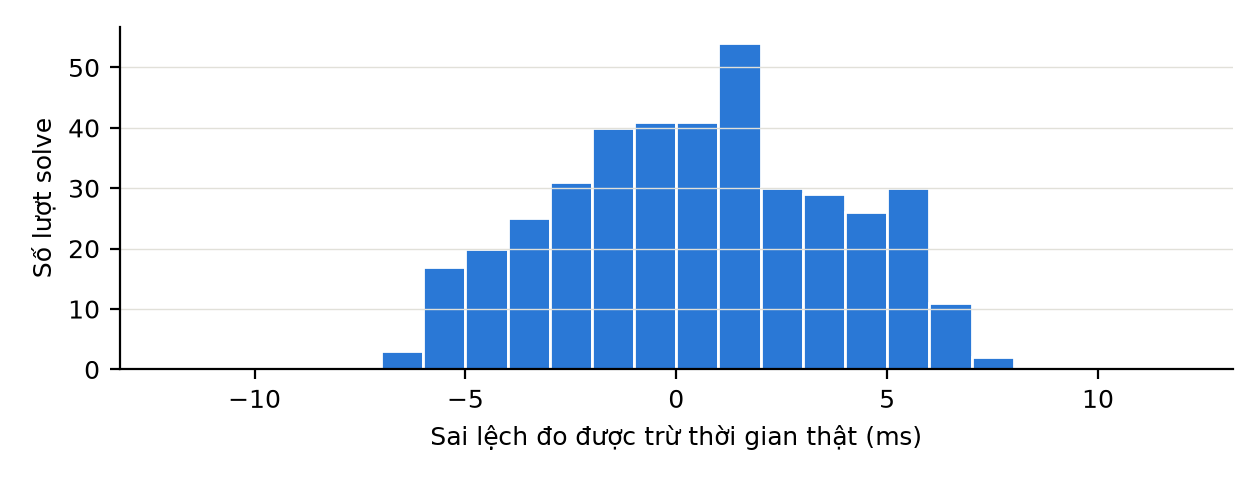
\includegraphics[width=0.92\textwidth]{figures/sim_timing.png}
    \caption{Sai lệch giữa thời gian đo được và thời gian thật trong 400 lượt solve mô phỏng}
    \label{fig:sim-timing}
\end{figure}

Con số này cần được đọc đúng với giả định của nó. Khoảng trễ 2 đến 10~ms mỗi cạnh là ước lượng từ báo cáo nghiên cứu nền, nên mô phỏng chỉ chứng minh rằng firmware không cộng thêm sai số nào ngoài độ trễ của cảm biến. Khi có thiết bị thật, nhóm sẽ thay mô hình bằng phép đo theo kế hoạch kiểm thử, và giữ nguyên cách phân tích này.

\section{Ablation các cơ chế thiết kế}
Mỗi cơ chế ở Chương~3 đều tốn một chút: vài byte trong bản ghi, một chỉ số, một quy tắc thứ tự hay một con chip. Để biết khoản tốn ấy có đáng không, nhóm lần lượt bỏ từng cơ chế khỏi mô phỏng, giữ nguyên mọi thứ khác, rồi chạy lại đúng kịch bản nhắm vào nó.

\begin{table}[H]
    \centering
    \small
    \renewcommand{\arraystretch}{1.35}
    \caption{Ablation cơ chế trong mô phỏng, tệp \texttt{code/sim/run\_ablations.py}}
    \label{tab:sim-ablation}
    \begin{tabular}{>{\bfseries\raggedright\arraybackslash}m{0.6cm} >{\raggedright\arraybackslash}m{3.6cm} >{\raggedright\arraybackslash}m{2.9cm} >{\raggedright\arraybackslash}m{4.4cm} >{\raggedright\arraybackslash}m{1.6cm}}
        \toprule
        \rowcolor{haitayblue}
        \textcolor{white}{Mã} & \textcolor{white}{Cơ chế bị bỏ} & \textcolor{white}{Có cơ chế} & \textcolor{white}{Bỏ cơ chế} & \textcolor{white}{Vi phạm} \\
        \midrule
        \rowcolor{haitayblue!8}
        A1 & Chống nảy ba mẫu, thay bằng một mẫu & 0/200 lượt đo sai & 198/200 lượt đo sai, do mẫu chập chờn làm đồng hồ chạy hoặc dừng nhầm & N2, N3 \\
        A2 & Thứ tự COMMIT rồi mới ACK & Mất 0 bản ghi & Mất 11 bản ghi, đúng một khung, khi dịch vụ dừng giữa ACK và COMMIT & N5 \\
        \rowcolor{haitayblue!8}
        A3 & Bản ghi sửa ghi thêm, thay bằng sửa tại chỗ & 0 lượt đã chốt bị mất qua 200 lần cắt điện & 28 lượt đã chốt bị mất qua 200 lần cắt điện & N4 \\
        A4 & CRC16 trong bản ghi & 184 lần ghi dở đều bị chặn & 184 bản ghi rác được nhận là hợp lệ & N4 \\
        \rowcolor{haitayblue!8}
        A5 & Khóa \texttt{(device\_id, seq)} & 0 bản ghi trùng & 11 bản ghi trùng sau khi rơi kết nối và mất ACK & N5 \\
        A6 & DS3231, chỉ đặt giờ bằng \texttt{SET\_TIME} & Mốc giờ được giữ khi rút cáp & 20/20 mốc giờ phải ước lượng khi rút cáp trước lúc đồng bộ & Mốc giờ thực \\
        \bottomrule
    \end{tabular}
\end{table}

Con số của A3 khớp với lập luận ở Chương~3. Khi sửa tại chỗ, 13 byte đầu không đổi, nên lần cắt điện chỉ gây hại khi rơi vào byte \texttt{flags} hoặc hai byte CRC, tức khoảng 2 trên 16 vị trí. Tỉ lệ đo được là 28 trên 200, xấp xỉ 14\%, sát với mức 12,5\% dự đoán. Kịch bản A1 là trường hợp xấu nhất, vì mô hình chèn một mẫu chập chờn vào mọi cạnh chạm và nhả.

Kết quả cho thấy thiết kế đang nằm ở điểm tối thiểu đủ dùng. Mỗi cơ chế có giá gần như bằng không, riêng DS3231 khoảng 44.000 đồng, và bỏ bất kỳ cơ chế nào đều làm vỡ một yêu cầu bắt buộc. Vì vậy nhóm giữ cả sáu cơ chế và không thêm cơ chế nào ngoài chúng.

\section{Dữ liệu mẫu và dashboard}
Kịch bản D1 tạo ra một người chơi luyện tập 90 ngày liền, mỗi ngày 15 đến 60 lượt. Thời gian trung bình giảm dần từ khoảng 26 giây xuống 18 giây, với 3\% lượt bị +2 và 2\% lượt DNF. Mỗi buổi tối thiết bị ảo đồng bộ qua đúng giao thức thật, nên bộ dữ liệu này đã đi qua toàn bộ luồng chứ không được chèn thẳng vào cơ sở dữ liệu.

\begin{figure}[H]
    \centering
    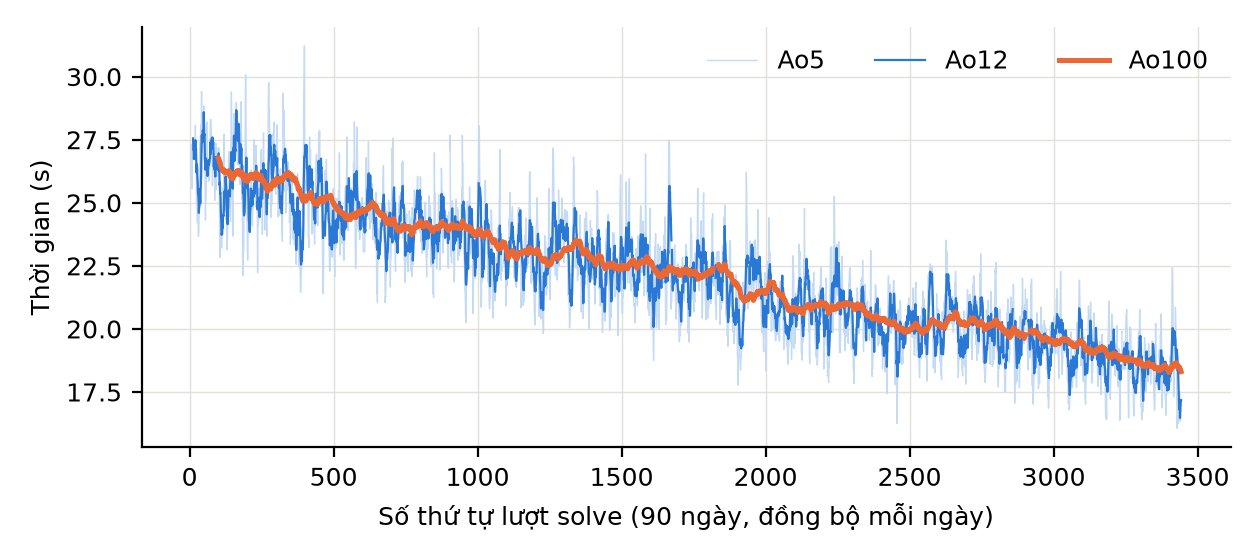
\includegraphics[width=0.92\textwidth]{figures/sim_rolling.png}
    \caption{Ao5, Ao12 và Ao100 truy vấn từ SQLite sau 90 ngày đồng bộ mô phỏng}
    \label{fig:sim-rolling}
\end{figure}

Hình~\ref{fig:sim-rolling} được vẽ từ chính hàm truy vấn mà điểm cuối \texttt{/stats/rolling} sẽ dùng. Ao5 dao động mạnh theo từng buổi, Ao12 mượt hơn, còn Ao100 cho thấy rõ xu hướng tiến bộ. Đây đúng là lý do dashboard đặt ba đường trên cùng một trục: người chơi vừa thấy phong độ hôm nay, vừa thấy hướng đi của cả quý. Ở giai đoạn này hình được xuất ra tệp tĩnh, và dashboard web sẽ dùng lại bộ dữ liệu mẫu này khi trình diễn.

\section{Đánh giá và bước tiếp theo}
Mô phỏng đã trả lời được câu hỏi lớn nhất của giai đoạn thiết kế: luồng dữ liệu có giữ được dữ liệu qua sự cố hay không. Những gì còn lại là câu hỏi về phần cứng, và chúng cần thiết bị thật để trả lời.

\begin{table}[H]
    \centering
    \small
    \renewcommand{\arraystretch}{1.4}
    \caption{Điều mô phỏng đã khẳng định và việc chuyển sang phần cứng}
    \label{tab:sim-next}
    \begin{tabular}{>{\bfseries\raggedright\arraybackslash}m{3.0cm} >{\raggedright\arraybackslash}m{5.4cm} >{\raggedright\arraybackslash}m{5.8cm}}
        \toprule
        \rowcolor{haitayblue}
        \textcolor{white}{Hạng mục} & \textcolor{white}{Mô phỏng đã khẳng định} & \textcolor{white}{Bước tiếp theo trên thiết bị thật} \\
        \midrule
        \rowcolor{haitayblue!8}
        Đo giờ & Firmware không thêm sai số ngoài độ trễ cảm biến; chạm ngắn không kích hoạt & Đo độ trễ thật bằng máy phân tích logic và camera 240 hình mỗi giây \\
        Lưu trữ & Không mất bản ghi đã chốt qua 100 lần cắt điện & Lặp lại 50 đến 100 lần cắt điện bằng relay trên FRAM thật \\
        \rowcolor{haitayblue!8}
        Đồng bộ & Không mất, không trùng qua rơi kết nối, khung hỏng, mất ACK & Đo thông lượng và tỉ lệ rơi kết nối với bleak trên máy tính trình diễn \\
        Máy tính & Lược đồ, quy đổi giờ, gắn người dùng, truy vấn Ao chạy đúng & Bọc \texttt{PcService} bằng FastAPI theo Bảng~\ref{tab:api}, nối dashboard Chart.js \\
        \bottomrule
    \end{tabular}
\end{table}

Thứ tự tiếp theo vì vậy đã rõ. Nhóm chuyển \texttt{proto}, \texttt{stats} và logic vòng đệm sang C trong ESP-IDF, giữ \texttt{run\_scenarios.py} làm bộ kiểm thử hồi quy cho phía máy tính. Khi bo mạch chạy được đường đo giờ, cùng các kịch bản này sẽ được chạy lại với thiết bị thật đứng ở đầu luồng.
